\glsreset{clf}\glsreset{cbf}
This chapter ought to lay the basics of all shared control theory applied in the following chapters dealing with the design of a safe controller.

Based on \citep{bib:artstein}, who founded \glspl{clf}, a \gls{cbf} can be created \citep{bib:org_control}. 
\begin{exa}[Control Barrier Function]
Given a system $\dot{x}=f(x)+g(x)u$, a \gls{cbf} exists if the below constraints are fulfilled:
\begin{subequations}
\begin{flalign}
x\in \mathcal{X}_u \hspace{0.3cm} &\Rightarrow \hspace{0.3cm} B(x) > 0  \label{req1} \\
L_gB(x) = 0 \hspace{0.3cm} &\Rightarrow \hspace{0.3cm} L_fB(x) < 0 \label{req2} \\
\{ x \in \mathcal{X} | B(x) \leq 0 \} &\neq \emptyset \label{req3}
\end{flalign}
\end{subequations}
\vspace{-0.6cm}
\begin{tabular}{r l l} 
where  & & \\
$B(x)$ & is a control barrier function & [$\cdot$] \\ 
$L_fB(x)$ & is the Lie derivative of $B(x)$ along the vector field  $f(x)$, i.e. $\frac{\partial B(x)}{\partial x}f(x)$ & [$\cdot$] \\ 
$L_gB(x)$ & is the Lie derivative of $B(x)$ along the vector field  $g(x)$, i.e. $\frac{\partial B(x)}{\partial x}g(x)$ & [$\cdot$] 
\end{tabular}
\vspace*{-0.2cm}
\end{exa}
Taking a look at \autoref{req1} it states essentially the same as \autoref{cer2}, i.e. the unsafe area exist whenever $B(x)>0$. This makes it possible to design an unsafe region. \Autoref{req2} put forth the requirement that the gradient along the vector field $f(x)$ must point away from the barrier extremities whenever the input is with no significance (except for the critical point). \Autoref{req3} simply states that the safe area must contain some states as control otherwise is impossible.

\section{The Control Law}\label{eq:control_for_safety}
A control law is now introduced:
\begin{flalign*}
u(x) =
\begin{cases}
	\bar{N}\,x_\text{ref} - K\,x \kk &\text{if \mm $x \in [\Lambda_{s-}:\Lambda_{s+}]$}\\
	 k_0(x)  \kk &\text{if \mm $x \in [\Lambda_{s+}:\Lambda_{h+}] \mm \wedge \mm x \in [\Lambda_{h-}:\Lambda_{s-}]$}
\end{cases}
\end{flalign*}
This can be combined by the control law below which is a linear combination of the two controllers.
\begin{flalign}
u(x) &= \sigma(x)k_0(x)+(1-\sigma(x))\tilde{u}(x) \nonumber \\
 &= \sigma(x)k_0(x)+(1-\sigma(x))(\bar{N} \cdot x_\text{ref}-Kx) \label{eq:control_law}
\end{flalign}
\vspace{-0.8cm}
\begin{longtable}{p{.9\textwidth} p{.1\textwidth} p{.1\textwidth}} 
Where  & & \\
$u(x) \in \mathbb{R}^{1 \times 1} $ is a control signal where safety is ensured  & [$\cdot$] \\
$\tilde{u}(x) \in \mathbb{R}^{1 \times 1}$ is a control signal to the linear state space system such that $\tilde{u}=\bar{N}\cdot x_\text{ref}-Kx $ & [$\cdot$] \\ 
$k_0(x) \in \mathbb{R}^{1 \times 1}$ is a control law that guarantees safety & [$\cdot$] \\ 
$\sigma(x) \in \mathbb{R}^{1 \times 1}$ is a parameter that founds a linear combination between the two control inputs & [$\cdot$] \\ 
$K \in \mathbb{R}^{1 \times n}$ is a constant feedback matrix where $n$ is the number of states & [$\cdot$] \\
$\bar{N} \in \mathbb{R}^{1 \times 1}$ is a constant to ensure unity gain from reference to output & [$\cdot$] \\
$x \in \mathbb{R}^{n \times 1}$ is the state vector& [m] 
\end{longtable}
\vspace*{-0.2cm}
The control law is thereby a linear combination of two controllers. It is noted that:
\begin{flalign*}
\sigma(x) = 
\begin{cases}
0 \mm &\Rightarrow \mm \text{Pure control by pole placement, i.e. $u(x) = \tilde{u}(x) =  \bar{N}\cdot x_\text{ref}-Kx$ } \\
1 \mm &\Rightarrow \mm \text{Pure control for safety i.e. $u(x) = k_0(x)$ }
\end{cases}
\end{flalign*}
The interval between 0 and 1 can be refined such that the transition between the two control laws is not instantaneous. This smoothing can be performed with a continuous approximation of the unit step of $B(x)$ by introducing a scalar $\epsilon>0$ \citep{bib:org_control}:
\begin{flalign}
\sigma(x) = 
\begin{cases}
0 & \text{if} \mm B(x) \leq -\epsilon \\
-2  \left( \dfrac{B(x)}{\epsilon} \right)^3 - 3\left( \dfrac{B(x)}{\epsilon} \right)^2 +1 \kk &\text{if} \mm B(x) \in (-\epsilon,0) \\
1  &\text{if} \mm B(x) \geq 0
\end{cases}
\label{eq:smoothness}
\end{flalign} 
%
%
% 
A block diagram is depicted in \autoref{fig:controlsystem}.
\begin{figure}[H]
	\center
		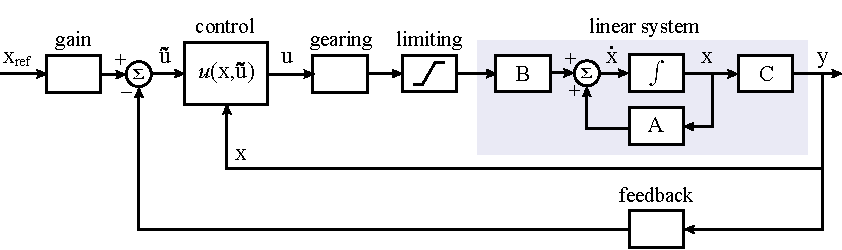
\includegraphics[scale=1]{control_system.pdf}
	\caption{Block diagram of the control system for slide position. MATLAB implementation is found in \autoref{app:slide_implement_1}. \color{green}{A,B,C matricerne skal skrives generelt i stedet for 1D tilf\ae ldet.}}
	\label{fig:controlsystem}
\end{figure}
\subsection*{Uniform Construction of $k_0$}
The control law ensuring safety can be found as \citep{bib:org_control}:
\begin{flalign}
k_0(x) = \begin{cases}
-\dfrac{L_fB(x)+ \sqrt{(L_fB(x))^2 + \kappa^2L_gB(x)(L_gB(x))^T}}{L_gB(x)(L_gB(x))^T}(L_gB(x))^T &\text{if} \mm L_gB(x) \neq 0 \\
0  &\text{if} \mm L_gB(x) = 0
\end{cases}
\label{eq:control_law}
\end{flalign}
$\kappa$ is a design variable. High values of $\kappa$ implies increased aggressiveness. \Autoref{eq:control_law} indeed ensures safety for the closed loop system $\dot{x} = f(x)+g(x)k_0(x)$. This is easily proven as:
\begin{flalign*}
L_{f_{cl}}B(x) = L_fB(x) + L_gB(x)k_0(x)
\end{flalign*}
For $L_gB(x) \neq 0:$
\begin{flalign*}
L_{f_{cl}}B(x) &= L_fB(x) + L_gB(x) \left( -\dfrac{L_fB(x)+ \sqrt{(L_fB(x))^2 + \kappa^2L_gB(x)(L_gB(x))^T}}{L_gB(x)(L_gB(x))^T}(L_gB(x))^T \right)  \\
&= L_fB(x) - L_gB(x)(L_gB(x))^T \dfrac{L_fB(x) + \sqrt{(L_fB(x))^2 + \kappa^2L_gB(x)(L_gB(x))^T}}{L_gB(x)(L_gB(x))^T}   \\ 
&= L_fB(x) - L_fB(x) - \sqrt{(L_fB(x))^2 + \kappa^2L_gB(x)(L_gB(x))^T} \\
&= - \sqrt{(L_fB(x))^2 + \kappa^2 L_gB(x)(L_gB(x))^T} \mm \leq 0 \mm \forall \mm x
\end{flalign*}
As all terms within the square root are squared, no imaginary numbers occur, as a result $L_{f_{cl}}B(x) \leq 0$ 

According to \autoref{eq:control_law}, when $L_gB(x) = 0$:
\begin{flalign*}
L_{f_{cl}}B(x) = L_fB(x) + L_gB(x)\cdot 0 = L_fB(x)
\end{flalign*}
As $L_fB(x)$ is constructed such that $L_gB(x) = 0 \hspace{0.15cm} \Rightarrow \hspace{0.15cm} L_fB(x) < 0 $ it is verified that $Lf_{cl}B(x)\leq 0 \,\,\forall x \in\mathcal{X}$. 
